\documentclass[../Cours.tex]{subfiles}

\begin{document}

\chapitre{Triangles}

\partie{Constructions}

\definition{Un triangle est une figure plane formée par 3 points et les segments qui les relient.}

\propriete{La somme des angles internes d'un triangle vaut \ang{180}.}

\souspartie{Avec trois longueurs}

\exemple{
\begin{align*}
    \mbox{on donne~~}&AB=\qty{4}{\centi\metre}\\
    &BC=\qty{5}{\centi\metre}\\
    &AC=\qty{6}{\centi\metre}
\end{align*}
\begin{itemize}
    \item[$\rightarrow$] on trace le côté le plus long 
    \item[$\rightarrow$] avec le compas, on trace les deux arcs de cercle correspondant aux deux côtés restants
    \item[$\rightarrow$] l'intersection des arcs de cercle sera le troisième sommet du triangle ; on le relie aux deux autres
\end{itemize}
\begin{center}
    \color{black}
    \begin{tikzpicture}
        \draw (0,0) node[left]{$A$} -- (6,0) node[right]{$C$};
        \draw[white] (4,0) arc(0:50:4) coordinate(arc1);
        \draw[dashed] (arc1) arc(50:70:4);
        \draw[white] (1,0) arc(180:150:5) coordinate (arc2);
        \draw[dashed] (arc2) arc(150:130:5);
        \draw[fill=black] (2.27,3.3) circle (0.04);
        \draw (0,0) -- ($({4*cos(55.5)},{4*sin(55.5)})$);
        \draw (6,0) -- ($(6,0)+({5*cos(138.6)},{5*sin(138.6)})$) node[above]{$B$};
    \end{tikzpicture}
\end{center}}

\clearpage
\souspartie{Avec 2 longueurs et 1 angle}

\paragraphe{noir}{Condition}{Il faut les longueurs de deux côtés du triangle et la mesure de l'angle formé par ces deux côtés.}

\exemple{
\begin{align*}
    \mbox{on donne~~}&AB=\qty{2}{\centi\metre}\\
    &BC=\qty{3}{\centi\metre}\\
    &\widehat{ABC}=\ang{60}
\end{align*}
\begin{itemize}
    \item[$\rightarrow$] on trace le plus grand côté
    \item[$\rightarrow$] on trace l'angle donné
    \item[$\rightarrow$] on reporte la longueur du deuxième côté
    \item[$\rightarrow$] on relie les sommets du triangle
\end{itemize}
\begin{center}
    \color{black}
    \begin{tikzpicture}[scale=1.5]
        \draw (0,0) node[left]{$B$} -- (3,0) node[right]{$C$};
        \draw (0.2,0) arc(0:60:0.2);
        \node[below] at (1.5,0) {\small{\qty{3}{\centi\metre}}};
        \node[above right] at (0.1,0) {\small{\ang{60}}};
        \draw[dashed] (0,0) -- ($({2.5*cos(60)},{2.5*sin(60)})$);
        \draw[latex-latex] (-0.1,0.1) -- ++($({2*cos(60)},{2*sin(60)})$);
        \draw[fill=black] ($({2*cos(60)},{2*sin(60)})$) circle (0.025);
        \node[rotate=60] at (0.2,1) {\small{\qty{2}{\centi\metre}}};
        \draw ($({2*cos(60)},{2*sin(60)})$) node[above]{$A$} --  (3,0);
    \end{tikzpicture}
\end{center}
}

\souspartie{Avec 1 longueur et 2 angles}
\paragraphe{noir}{Condition}{Il faut la longueur d'un côté et les 2 angles adjacents à ce côté (les 2 angles qui touchent ce côté).}

\remarque{À partir de deux angles, je peux obtenir le troisième.}

\exemple{
\begin{align*}
    \mbox{on donne~~}&DF=\qty{4}{\centi\metre}\\
    &\widehat{EDF}=\ang{45}\\
    &\widehat{DFE}=\ang{90}
\end{align*}
\begin{itemize}
    \item[$\rightarrow$] on trace le côté
    \item[$\rightarrow$] on trace les deux demi-droites qui permettent de former les 2 angles
    \item[$\rightarrow$] le troisième sommet du triangle est le point d'intersection des deux demi-droites
\end{itemize}
\begin{center}
    \color{black}
    \begin{tikzpicture}
        \draw (0,0) node[left]{$D$} -- (4,0) node[right]{$F$};
        \draw[dashed] (0,0) -- (5,5);
        \draw[dashed] (4,0) -- (4,5);
        \draw[fill=black] (4,4) circle (0.05) node[right]{$E$};
        \node[below] at (2,0) {\qty{4}{\centi\metre}};
        \draw (0.5,0) arc(0:45:0.5);
        \draw[fill=black] (4,0) rectangle (3.8,0.2);
        \node[right] at (0.5,0.3) {\ang{45}};
    \end{tikzpicture}
\end{center}
}

\clearpage

\partie{Nomenclature des triangles}
\souspartie{Triangle isocèle}

\definition{Un triangle isocèle est un triangle qui a deux côtés de même longueur.}
\illustration{
\begin{center}
    \begin{tikzpicture}
        \draw (0,1.5) node[above]{$B$} -- (-2,0) node[left]{$A$} -- (2,0) node[right]{$C$} -- cycle;
        \node[rotate=30] at (-1,0.7) {\small{||}};
        \node[rotate=-30] at (1,0.7) {\small{||}};
        \draw[fill=rouge,rouge] ($(-2,0)+(0.5,0)$) arc (0:37:0.5) -- (-2,0) -- cycle;
        \draw[fill=rouge,rouge] ($(2,0)+(-0.5,0)$) arc (180:143:0.5) -- (2,0) -- cycle;
        \draw[latex-] (0.1,1.5) -- (1.3,1.5) node[anchor=west,right]{\small{sommet principal}};
        \draw[latex-] (-0.5,-0.15) arc (120:250:0.25) node[right, anchor=west] {\small{la base}};
    \end{tikzpicture}
\end{center}
Le triangle $ABC$ est isocèle \underline{en $B$} car $BA=BC$.
}

\propriete{Les deux angles adjacents à la base sont égaux.}
\exemple{Sur le schéma précédent : $\widehat{BAC}=\widehat{BCA}$.}

\souspartie{Triangle rectangle}

\definition{Un triangle rectangle est un triangle qui possède un angle droit (=~\ang{90}).}

\illustration{
\begin{center}
    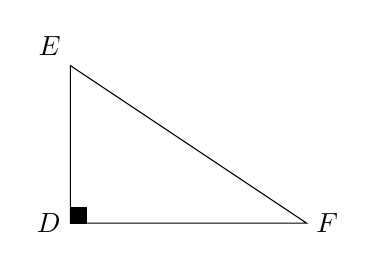
\begin{tikzpicture}
        \draw (0,0) node[right]{$F$} -- (-3,0) node[left]{$D$} -- (-3,2) node[above left]{$E$} -- cycle;
        \draw[fill=black] (-3,0) rectangle (-2.8,0.2);
    \end{tikzpicture}
\end{center}
Le triangle $DEF$ est rectangle \underline{en D}.}


\clearpage
\souspartie{Triangle équilatéral}

\definition{Un triangle équilatéral a ses trois côtés de même longueur.}

\begin{center}
    \begin{tikzpicture}
        \draw (0,0) node[left]{$G$} -- ($({3*cos(60)},{3*sin(60)})$) node[above]{$H$} -- (3,0) node[right]{$I$} -- cycle;
        \node[rouge,rotate=-30] at ($({1.5*cos(60)},{1.5*sin(60)})$) {s};
        \node[rouge,rotate=30] at ($(3,0)+({-1.5*cos(60)},{1.5*sin(60)})$) {s};
        \node[rouge,rotate=90] at (1.5,0) {s};
        %\draw[rouge,fill=rouge] (0.3,0) arc (0:60:0.3) -- (0,0) -- cycle;
        %\draw[rouge,fill=rouge] (2.7,0) arc (180:120:0.3) -- (3,0) -- cycle;
        %\draw[rouge,fill=rouge] ($({2.7*cos(60)},{2.7*sin(60)})$) arc (-120:-60:0.3) -- ($({3*cos(60)},{3*sin(60)})$) -- cycle;
    \end{tikzpicture}
\end{center}

\propriete{Tous les angles d'un triangle équilatéral ont la même mesure : $\dfrac{180}{3} = \ang{60}.$}

\souspartie{Autres cas}
\illustration{
\begin{center}
    \begin{tikzpicture}
        \draw (-1,0) node[right]{$L$} -- (-3,0) node[left]{$K$} -- (-3,2) node[above left]{$J$} -- cycle;
        \draw[fill=black] (-3,0) rectangle (-2.8,0.2);
        \node[rotate=90,rouge] at (-3,1) {\small{||}};
        \node[rouge] at (-2,0) {\small{||}};
    \end{tikzpicture}
\end{center}
$JKL$ est un triangle rectangle et isocèle \underline{en K} car : $\widehat{JKL}$ est un angle droit et $KJ=KL$.
}

\propriete{Dans un triangle isocèle rectangle, les angles adjacents à la base valent \ang{45}.}
\remarque{Un triangle qui n'a aucune particularité est dit \underline{quelconque}.}

\end{document}

\clearpage
\partie{Droites remarquables dans un triangle}

\souspartie{Médiatrices}

\definition{La médiatrice d'un segment est la droite qui coupe le segment en son milieu perpendiculairement.}

\illustration{\vspace{-1cm}
\begin{center}
\begin{tikzpicture}
    \draw (0,0) -- (4,0);
    \draw[fill=noir] (0,0) node[below] {$A$} circle (0.05);
    \draw[fill=noir] (4,0) node[below] {$B$} circle (0.05);
    \draw[red] (2,-1.5) -- (2,2);
    \draw[fill=noir] (2,0) rectangle (2.15,0.15);
    \node[rouge] at (1,0) {||};
    \node[rouge] at (3,0) {||};
\end{tikzpicture}
\end{center}
}

\remarque{Dans un triangle, il y a 3 médiatrices.}

\illustration{\vspace{-1cm}
\begin{center}
\begin{tikzpicture}
    \draw[red] (0,0) -- (4,0);
    \draw[dashed,red] (2,-1) -- (2,2);
    \draw[blue] (4,0) -- (3,2);
    \draw[dashed,blue] (3.5,1) -- ++(27:1);
    \draw[dashed,blue] (3.5,1) -- ++(-153:2.5);
    \draw[vert] (3,2) -- (0,0);
    \draw[dashed,vert] (1.5,1) -- ++(123:1);
    \draw[dashed,vert] (1.5,1) -- ++(-57:1.5);
\end{tikzpicture}
\end{center}
}

\propriete{Les trois médiatrices d'un triangle concourent en un point appelé le centre du cercle circonscrit.}

\consequence{Dans un triangle $ABC$, si $M$ est le centre du cercle circonscrit : $$MA = MB = MC$$}

\vspace{-1cm}
\illustration{\vspace{-1cm}
\begin{center}
\begin{tikzpicture}
    \draw[red] (0,0) node[left]{\textcolor{noir}{$A$}} -- (4,0);
    \draw[dashed,red] (2,-1) -- (2,2);
    \draw[blue] (4,0) node[right]{\textcolor{noir}{$B$}} -- (3,2);
    \draw[dashed,blue] (3.5,1) -- ++(27:1);
    \draw[dashed,blue] (3.5,1) -- ++(-153:2.5);
    \draw[vert] (3,2) node[above]{\textcolor{noir}{$C$}} -- (0,0);
    \draw[dashed,vert] (1.5,1) -- ++(123:1);
    \draw[dashed,vert] (1.5,1) -- ++(-57:1.5);
    \draw[fill=black] (2,0.25) circle (0.05);
    \draw (2,0.25) circle (2);
    \node[above right] at (2,0.25) {$M$};
\end{tikzpicture}
\end{center}
}

\souspartie{Hauteurs}

\definition{Dans un triangle, la hauteur d'un côté est la droite perpendiculaire à ce côté et qui passe par le sommet opposé.}

\illustration{\vspace{-1cm}
\begin{center}
\begin{tikzpicture}
    \draw (0,0) node[left]{$A$} -- (4,0) node[right]{$B$} -- (3,2) node[above right]{$C$} -- cycle;
    \draw[red,dashed] (3,-0.5) -- (3,2.5);
    \node[left,red] at (3,1) {$(d)$};
    \node[anchor=west] at (6,1.2) {$(d)$ est la hauteur issue de C.};
    \node[anchor=west] at (6,0.5) {$(d)$ est aussi la hauteur de $[AB]$.};
    \draw[fill=noir] (3,0) rectangle (3.2,0.2);
\end{tikzpicture}
\end{center}
\begin{center}
\begin{tikzpicture}
    \draw (0,0) node[left]{$M$} -- (4,0) node[right]{$N$} -- (1,3) node[above right]{$P$} -- cycle;
    \coordinate (A) at (0,0);
    \coordinate (H) at ($(4,0)!(0,0)!(1,3)$);
    \draw[red,dashed] ($(A)!-0.2!(H)$) -- ($(A)!1.2!(H)$);
    \node[below right,red] at (1,1) {$(d)$};
    \node[anchor=west] at (6,1.2) {$(d)$ est la hauteur issue de $M$.};
    \node[anchor=west] at (6,0.5) {$(d)$ est aussi la hauteur de $[NP]$.};
    \draw[rotate=135,fill=noir] (H) rectangle ($(H)+(0.2,0.2)$);
\end{tikzpicture}
\end{center}
}

\notation{Dans un triangle $ABC$, la hauteur du côté $[AB]$ se nomme aussi la hauteur issue de $C$.}

\propriete{Les trois hauteurs d'un triangle concourent en un point : l'orthocentre.}

\illustration{
\begin{center}
\begin{tikzpicture}[scale=1.5]
    \draw (0,0) node[left]{$A$} coordinate (A) -- (5,0) node[right]{$B$} coordinate (B) -- (1.5,3) node[above left]{$C$} coordinate (C) -- cycle;
    \coordinate (H) at ($(A)!(C)!(B)$);
    \coordinate (I) at ($(A)!(B)!(C)$);
    \coordinate (J) at ($(C)!(A)!(B)$);
    \draw[red, dashed] ($(C)!-0.2!(H)$) -- ($(C)!1.2!(H)$); 
    \draw[red, dashed] ($(B)!-0.2!(I)$) -- ($(B)!1.2!(I)$); 
    \draw[red, dashed] ($(A)!-0.2!(J)$) -- ($(A)!1.2!(J)$);
    \draw[fill=noir] (H) rectangle ($(H)+(0.15,0.15)$);
    \draw[fill=noir,rotate=-25] (I) rectangle ($(I)+(0.15,0.15)$);
    \draw[fill=noir,rotate=-132] (J) rectangle ($(J)+(0.15,0.15)$);
\end{tikzpicture}
\end{center}
}

\clearpage

\renewcommand\tabularxcolumn[1]{m{#1}}
\begin{tabularx}{\textwidth}{C|C}\hline
    \makecell{La hauteur du côté $[AB]$ \\ la hauteur issue de $C$} & 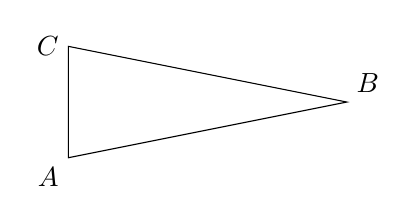
\begin{tikzpicture}[rotate=-45]
        \coordinate (A) at (0,0);
        \coordinate (B) at (2,3);
        \coordinate (C) at (-1,1);
        \draw (A) node[below left]{$A$} -- (B) node[above right]{$B$} -- (C) node[left]{$C$} -- cycle;
    \end{tikzpicture} \\\hline
    .... & \begin{tikzpicture}[rotate=-35]
        \coordinate (A) at (0,0);
        \coordinate (B) at (2,3);
        \coordinate (C) at (-1,1);
        \draw (A) node[below left]{$A$} -- (B) node[above right]{$B$} -- (C) node[left]{$C$} -- cycle;
        \coordinate (H) at ($(B)!(A)!(C)$);
        \draw[dashed] ($(A)!-0.2!(H)$) -- ($(A)!1.5!(H)$);
    \end{tikzpicture} \\\hline
    .... & \begin{tikzpicture}[rotate=-35]
        \coordinate (A) at (0,0);
        \coordinate (B) at (3,2);
        \coordinate (C) at (-1,1);
        \draw (A) node[below left]{$A$} -- (B) node[above right]{$B$} -- (C) node[left]{$C$} -- cycle;
        \coordinate (I) at ($(B)!0.5!(C)$);
        \coordinate (v) at (1,-4);
        \draw[dashed] ($(I)-0.5*(v)$) -- ($(I)+0.5*(v)$);
    \end{tikzpicture} \\\hline
    La médiatrice de $[AC]$ & 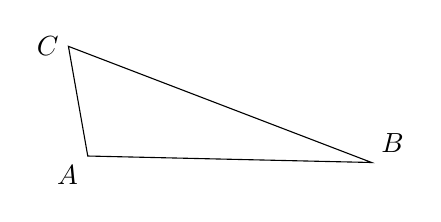
\begin{tikzpicture}[rotate=-35]
        \coordinate (A) at (0,0);
        \coordinate (B) at (3,2);
        \coordinate (C) at (-1,1);
        \draw (A) node[below left]{$A$} -- (B) node[above right]{$B$} -- (C) node[left]{$C$} -- cycle;
    \end{tikzpicture} \\\hline
    Les trois médiatrices de $ABC$ & \begin{tikzpicture}[rotate=-25]
        \coordinate (A) at (0,-1);
        \coordinate (B) at (3,1.5);
        \coordinate (C) at (-1,0);
        \draw (A) node[below left]{$A$} -- (B) node[above right]{$B$} -- (C) node[left]{$C$} -- cycle;
        \coordinate (I) at ($(B)!0.5!(C)$);
        \coordinate (v) at (1.5,-4);
        \draw[dashed] ($(I)-0.5*(v)$) -- ($(I)+0.5*(v)$);
    \end{tikzpicture} \\\hline
    Les trois hauteurs de $ABC$ & \begin{tikzpicture}[rotate=-25]
        \coordinate (A) at (-0.6,-1.8);
        \coordinate (B) at (3,1.5);
        \coordinate (C) at (-2,0);
        \draw (A) node[below left]{$A$} -- (B) node[above right]{$B$} -- (C) node[left]{$C$} -- cycle;
        \coordinate (H) at ($(B)!(A)!(C)$);
        \draw[dashed] ($(A)!-0.2!(H)$) -- ($(A)!1.5!(H)$);
    \end{tikzpicture} \\\hline
\end{tabularx}

\end{document}

